\documentclass[crop,tikz]{standalone}
\usepackage{amsmath}
\usepackage{amsfonts}
\usepackage{physics}
\usepackage{tikz}
\usetikzlibrary{shapes}
\usepackage{dsfont}
\usepackage{bbm}
% parameters for the MPS drawings
\definecolor{Tcolor}{RGB}{255, 235, 171}
\definecolor{Wcolor}{RGB}{190, 190, 255}
\def\textoffsetVertical{0.8}
\def\nodewidth{0.6*28.5}
\def\legwidth{0.8}
\def\nodedistance{1.25}
\def\textoffsetVerticalW{0.9}
\def\textoffsetHorizontalW{-0.9}
\def\textoffsetVerticalMPO{1.2}
\def\yoffset{1}
\def\xoffset{3}
\def\resultMPSYoffset{2.5}
\def\resultMPSXOffsetSmall{2}
\def\resultMPSXOffset{3}
\def\dotsOffset{3}
\def\conjOffsetVertical{1.25}
\def\conjOffsetVerticalLarge{2.2}
\def\curvedLineXOffset{0.7}
\def\cmscale{28.5}
\def\miniatureScale{0.5}
\def\Heffheight{1.2*28.5}
\def\Heffwidth{4.0*28.5}
\def\Heffonewidth{3.0*28.5}
\def\miniatureTextOffsetVertical{0.5}
\begin{document}
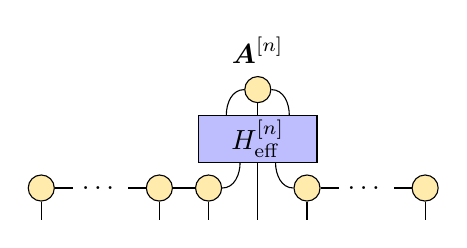
\begin{tikzpicture}[baseline=(current  bounding  box.center)]
    \node[draw, shape=circle, fill=Tcolor, minimum width=\nodewidth*\miniatureScale] (T1c) at (0, -\conjOffsetVertical*\miniatureScale) {};
    \node[draw, shape=circle, fill=Tcolor, minimum width=\nodewidth*\miniatureScale] (T2c) at ({(1*\dotsOffset)*\miniatureScale}, -\conjOffsetVertical*\miniatureScale) {};
    \node[draw, shape=circle, fill=Tcolor, minimum width=\nodewidth*\miniatureScale] (T3c) at ({(1*\nodedistance+1*\dotsOffset)*\miniatureScale}, -\conjOffsetVertical*\miniatureScale) {};
    \node[draw, shape=circle, fill=Tcolor, minimum width=\nodewidth*\miniatureScale] (T5c) at ({(3*\nodedistance+1*\dotsOffset)*\miniatureScale}, -\conjOffsetVertical*\miniatureScale) {};
    \node[draw, shape=circle, fill=Tcolor, minimum width=\nodewidth*\miniatureScale] (T6c) at ({(3*\nodedistance+2*\dotsOffset)*\miniatureScale}, -\conjOffsetVertical*\miniatureScale) {};

    \draw (T1c) -- ++(\legwidth*\miniatureScale, 0);
    \draw (T1c) -- ++(0, -\legwidth*\miniatureScale);
    \draw (T2c) -- ++(-\legwidth*\miniatureScale, 0);
    \draw (T2c) -- ++(0, -\legwidth*\miniatureScale);
    \draw (T2c) -- (T3c);
    \draw (T3c) -- ++(0, -\legwidth*\miniatureScale);
    \draw (T5c) -- ++(0, -\legwidth*\miniatureScale);
    \draw (T5c) -- ++(\legwidth*\miniatureScale, 0);
    \draw (T6c) -- ++(0, -\legwidth*\miniatureScale);
    \draw (T6c) -- ++(-\legwidth*\miniatureScale, 0);

    \node[] (dots1) at (\dotsOffset/2*\miniatureScale, -\conjOffsetVertical*\miniatureScale) {$\dots$};
    \node[] (dots1) at ({(3*\nodedistance+1.5*\dotsOffset)*\miniatureScale}, -\conjOffsetVertical*\miniatureScale) {$\dots$};

    \draw[] (T3c) to[in=-90, out=0] (\nodedistance*\miniatureScale+\dotsOffset*\miniatureScale+\legwidth*\miniatureScale, -\Heffheight/\cmscale/2*\miniatureScale);
    \draw[] (T5c) to[in=-90, out=180] (3*\nodedistance*\miniatureScale+\dotsOffset*\miniatureScale-\legwidth*\miniatureScale, -\Heffheight/\cmscale/2*\miniatureScale);
    \draw[] ({(2*\nodedistance+1*\dotsOffset)*\miniatureScale}, -\Heffheight/\cmscale/2*\miniatureScale) to[] ({(2*\nodedistance+1*\dotsOffset)*\miniatureScale}, -\conjOffsetVertical*\miniatureScale-\legwidth*\miniatureScale);

    % MPO
    %\node[draw, shape=rectangle, fill=Wcolor, minimum width=\nodedistance*100*\miniatureScale, minimum height=\nodewidth*\miniatureScale] (Heff) at ({(\dotsOffset+2.5*\nodedistance)*\miniatureScale}, 0) {$H_\text{eff,2}$};
    \node[draw, shape=rectangle, fill=Wcolor, minimum width=\Heffonewidth*\miniatureScale, minimum height=\Heffheight*\miniatureScale, inner sep=0] (Heff) at ({(\dotsOffset+2*\nodedistance)*\miniatureScale}, 0) {$H_\text{eff}^{[n]}$};

    \node[draw, shape=circle, fill=Tcolor, minimum width=\nodewidth*\miniatureScale] (A) at ({(\dotsOffset+2*\nodedistance)*\miniatureScale}, \conjOffsetVertical*\miniatureScale) {};
    \node[] (Atext) at ({(\dotsOffset+2*\nodedistance)*\miniatureScale}, \conjOffsetVertical*\miniatureScale+\miniatureTextOffsetVertical) {$\vb*{A}^{[n]}$};

    \draw[] (A) to[] ({(2*\nodedistance+1*\dotsOffset)*\miniatureScale}, \Heffheight/\cmscale/2*\miniatureScale);
    \draw[] (A.east) to[in=90, out=0] (2*\nodedistance*\miniatureScale+1*\dotsOffset*\miniatureScale+\legwidth*\miniatureScale, \Heffheight/\cmscale/2*\miniatureScale);
    \draw[] (A.west) to[in=90, out=180] (2*\nodedistance*\miniatureScale+1*\dotsOffset*\miniatureScale-\legwidth*\miniatureScale, \Heffheight/\cmscale/2*\miniatureScale);

\end{tikzpicture}
\end{document}